\section{Voronoi Diagrams}

Voronoi diagrams are a set of techniques used to partition a plane into $n$ regions (called Voronoi cells).
This is done by first scattering $n$ nodes, referred to as \textit{seeds}, onto the plane.
Subsequently, each seed is assigned its own region and all points on the plane will be assigned to the region of the closest seed.
These regions can then be used in PCG-scenarios such as dividing land areas into regions with less obvious patterns than those formed by using a simple grid.
Another use case is to reduce memory consumption through seamless chunk loading, not unlike \textit{Minecraft} \cite{minecraft}.

\begin{figure}[H]
  \centering
  \begin{subfigure}[b]{0.4\textwidth}
    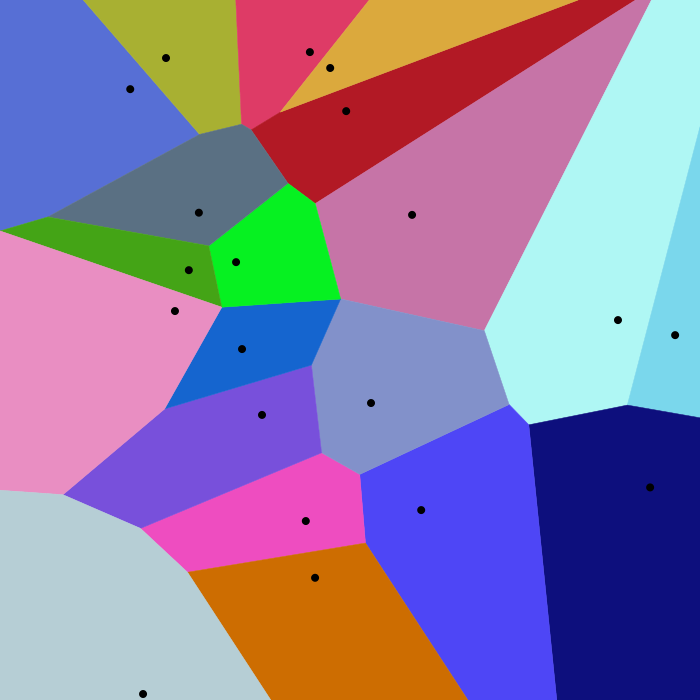
\includegraphics[width=\linewidth]{figure/voronoi_euclidean.png}
    \caption{Voronoi diagram using Euclidean distance \cite{voronoi_euclidean}.}
    \label{fig:voronoi_euclidean}
  \end{subfigure}
  ~
  \begin{subfigure}[b]{0.4\textwidth}
    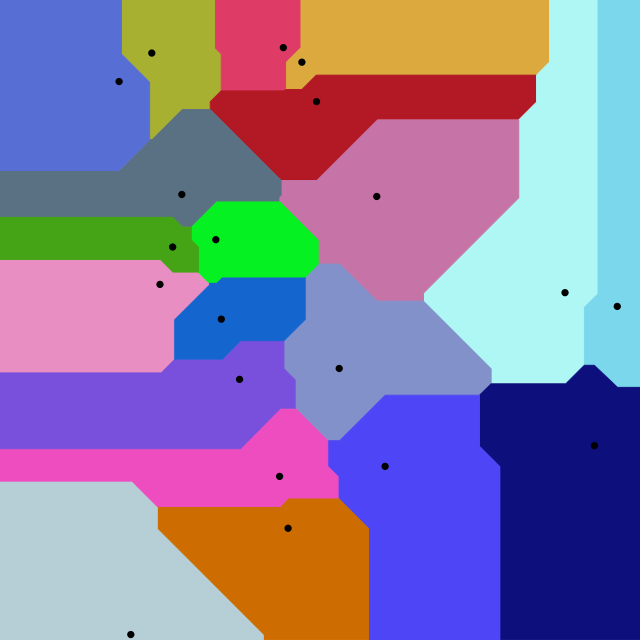
\includegraphics[width=\linewidth]{figure/voronoi_manhattan.png}
    \caption{Voronoi diagram using Manhattan distance \cite{voronoi_manhattan}.}
    \label{fig:voronoi_manhattan}
  \end{subfigure}
  \caption{Voronoi diagrams using identical seeds but different distance metrics.}
  \label{fig:voronoi}
\end{figure}
\vspace{-0.5cm} % Bad practice

Voronoi diagrams can be visualized by marking seeds with black dots and by coloring each regions' points with a unique color (see examples in figure \ref{fig:voronoi}).
The construction of these diagrams can be implemented using either Lloyd's Algorithm \cite{voronoi_lloyd}, or Fortune's Algorithm \cite{voronoi_fortune}. 